\documentclass[12pt]{article}%
\usepackage{amsmath}
\usepackage{amsfonts}
\usepackage{amssymb}
\usepackage{graphicx}%
\setcounter{MaxMatrixCols}{30}
%TCIDATA{OutputFilter=latex2.dll}
%TCIDATA{Version=5.50.0.2953}
%TCIDATA{CSTFile=40 LaTeX article.cst}
%TCIDATA{Created=Thursday, June 08, 2017 12:02:06}
%TCIDATA{LastRevised=Saturday, June 10, 2017 13:22:08}
%TCIDATA{<META NAME="GraphicsSave" CONTENT="32">}
%TCIDATA{<META NAME="SaveForMode" CONTENT="1">}
%TCIDATA{BibliographyScheme=Manual}
%TCIDATA{<META NAME="DocumentShell" CONTENT="Standard LaTeX\Blank - Standard LaTeX Article">}
%BeginMSIPreambleData
\providecommand{\U}[1]{\protect\rule{.1in}{.1in}}
%EndMSIPreambleData
\newtheorem{theorem}{Theorem}
\newtheorem{acknowledgement}[theorem]{Acknowledgement}
\newtheorem{algorithm}[theorem]{Algorithm}
\newtheorem{axiom}[theorem]{Axiom}
\newtheorem{case}[theorem]{Case}
\newtheorem{claim}[theorem]{Claim}
\newtheorem{conclusion}[theorem]{Conclusion}
\newtheorem{condition}[theorem]{Condition}
\newtheorem{conjecture}[theorem]{Conjecture}
\newtheorem{corollary}[theorem]{Corollary}
\newtheorem{criterion}[theorem]{Criterion}
\newtheorem{definition}[theorem]{Definition}
\newtheorem{example}[theorem]{Example}
\newtheorem{exercise}[theorem]{Exercise}
\newtheorem{lemma}[theorem]{Lemma}
\newtheorem{notation}[theorem]{Notation}
\newtheorem{problem}[theorem]{Problema}
\newtheorem{proposition}[theorem]{Proposition}
\newtheorem{remark}[theorem]{Remark}
\newtheorem{solution}[theorem]{Solution}
\newtheorem{summary}[theorem]{Summary}
\newenvironment{proof}[1][Proof]{\noindent\textbf{#1.} }{\ \rule{0.5em}{0.5em}}
\begin{document}
\section*{Subiectul 5}

\begin{problem}
\label{Gautschip4.31}Ecua\c{t}ia urm\u{a}toare se folose\c{s}te \^{\i}n
inginerie la determinarea vitezelor unghiulare critice pentru axe circulare:%
\[
f(x)=0,\quad f(x)=\tan x+\tanh x,~x>0.
\]


\begin{enumerate}
\item[(a)] Ar\u{a}ta\c{t}i c\u{a} are o infinitate de r\u{a}d\u{a}cini
pozitive, exact c\^{a}te una, $\alpha_{n}$, \^{\i}n fiecare interval de forma
$\left[  \left(  n-\frac{1}{2}\right)  \pi,n\pi\right]  $, $n=1,2,3,\dots$ (1p)

\item[(b)] Determina\c{t}i $\lim_{n\rightarrow\infty}\left(  n\pi-\alpha
_{n}\right)  $. (1p)

\item[(c)] Discuta\c{t}i convergen\c{t}a metodei lui Newton dac\u{a} se
porne\c{s}te cu $x_{0}=n\pi$. (2p)
\end{enumerate}
\end{problem}

\begin{proof}
[Solution]

\begin{enumerate}
\item[(a)] Graficele lui  $y=\tan x$ \c{s}i $y=-\tanh x$  se intersecteaz\u{a}
de o infinitate de ori pe $\mathbb{R}_{+}$, exact o dat\u{a} \^{\i}n fiecare
interval $[(n-1/2)\pi,n\pi]$, $n=1,2,3,\dots$. Abscisele respective
$\alpha_{n}$ sunt r\u{a}d\u{a}cinile pozitive ale ecua\c{t}iei (figura
\ref{figp31}).

\item[(b)] Deoarece $\tanh x\rightarrow1$ c\^{a}nd $x\rightarrow\infty$,
discu\c{t}ia de la (a) ne arat\u{a} c\u{a}  $\alpha_{n}-n\pi\sim\tan
^{-1}(-1)=-\tan^{-1}(1)$, deci $n\pi-\alpha_{n}\rightarrow\tan^{-1}(1)$
$=\pi/4=.785398\dots$ c\^{a}nd $n\rightarrow\infty$.

\item[(c)] Pe intervalul $I_{n}=\left[  (n-1/2)\pi,n\pi\right]  $ avem
$f\left(  (n-1/2)\pi\right)  =-\infty$, $f(n\pi)=\tanh n\pi>0$ \c{s}i%
\begin{align*}
f^{\prime}(x) &  =\tan^{2}x-\tanh^{2}x+2\\
f^{\prime\prime}(x) &  =2\tan x\left(  \tan^{2}x+1\right)  -2\tanh x\left(
1-\tanh^{2}x\right)
\end{align*}
Deci, $f$ este monoton cresc\u{a}toare \c{s}i concav\u{a} pe $I_{n}$. Metoda
lui Newton va converge dac\u{a} se porne\c{s}te cu cap\u{a}tul din dreapta,
$x_{0}=n\pi$, dac\u{a} $x_{1}>(n-1/2)\pi$. Deoarece func\c{t}ia $u/(2-u^{2})$
este cresc\u{a}toare pe $[0,1]$ \c{s}i ia valori \^{\i}ntre 0 \c{s}i 1, avem%
\[
x_{1}=n\pi-\frac{\tanh n\pi}{2-\tanh^{2}n\pi}>n\pi-1>n\pi-\frac{1}{2}\pi.
\]

\end{enumerate}
\end{proof}

\begin{figure}[ptbh]
\begin{center}
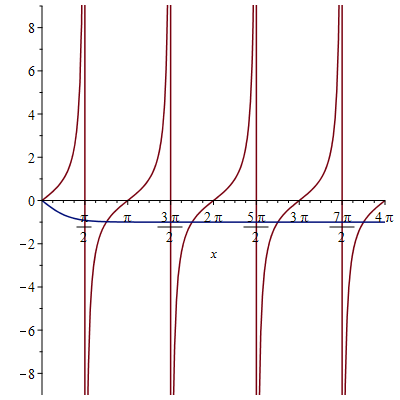
\includegraphics[
height=5.4235cm,
width=5.4235cm
]{tantanh.png}
\end{center}
\caption{Problema \ref{Gautschip4.31}}%
\label{figp31}%
\end{figure}

\begin{problem}


\begin{enumerate}
\item[(a)] Stabili\c{t}i o formul\u{a} de cuadratur\u{a} cu dou\u{a} noduri
\c{s}i cu grad maxim de exactitate
\[
\int_{0}^{1}\sqrt{x}f(x)\mathrm{d}\,x=A_{1}f(x_{1})+A_{2}f(x_{2})+R(f)
\]
reduc\^{a}nd cuadratura la o cuadratur\u{a} de tip Gauss-Jacobi. (3p)

\item[(b)] Folosind ideea de la (a), calcula\c{t}i
\[
\int_{0}^{1}\sqrt{x}\cos x\mathrm{d}\,x
\]
cu 8 zecimale exacte (2p)
\end{enumerate}
\end{problem}

\begin{proof}
[Solu\c{t}ie]

\begin{enumerate}
\item[(a)] Efectu\u{a}m schimbarea de variabil\u{a} $x=\frac{t+1}{2}$%
\[
\int_{0}^{1}\sqrt{x}\cos x\mathrm{d}\,x=\frac{\sqrt{2}}{4}\int_{-1}^{1}%
\sqrt{t+1}\cos\frac{t+1}{2}\,dt
\]
Cuadratura este de tip Gauss-Jacobi cu $\alpha=0$, $\beta=\frac{1}{2}$.
Polinomul ortogonal este%
\[
\pi_{2}(t)=t^{2}-\frac{2}{9}t-\frac{17}{63}%
\]
cu r\u{a}d\u{a}cinile $x_{1}=\frac{4}{63}\sqrt{70}+\frac{1}{9},x_{2}=\frac
{1}{9}-\frac{4}{63}\sqrt{70}$. Coeficien\c{t}ii%
\begin{align*}
A_{1}  & =\int_{-1}^{1}\frac{t-\left(  \frac{1}{9}-\frac{4}{63}\sqrt
{70}\right)  }{\frac{4}{63}\sqrt{70}+\frac{1}{9}-\left(  \frac{1}{9}-\frac
{4}{63}\sqrt{70}\right)  }\mathrm{d}\,t=1-\frac{1}{40}\sqrt{7}\sqrt{10}\\
A_{2}  & =\int_{-1}^{1}\frac{t-\left(  \frac{1}{9}+\frac{4}{63}\sqrt
{70}\right)  }{-\frac{4}{63}\sqrt{70}+\frac{1}{9}-\left(  \frac{1}{9}+\frac
{4}{63}\sqrt{70}\right)  }\mathrm{d}\,t=\frac{1}{40}\sqrt{7}\sqrt{10}+1
\end{align*}
Restul:%
\[
R(f)=\frac{f^{(4)}(\xi)}{4!}\int_{-1}^{1}\sqrt{t+1}\left(  t^{2}-\frac{2}%
{9}t-\frac{17}{63}\right)  ^{2}\mathrm{d}\,t=\frac{512}{130\,977}\sqrt
{2}f^{\left(  4\right)  }\left(  \xi\right)
\]


\item[(b)] 
\end{enumerate}
\end{proof}

\section*{Subiectul 6}

\begin{problem}
\label{Gautschip4.41}Ecua\c{t}ia $f(x)=x^{2}-3x+2=0$ are r\u{a}d\u{a}cinile 1
\c{s}i 2. Scris\u{a} sub forma de punct fix, $x=\frac{1}{\omega}\left[
x^{2}-\left(  3-\omega\right)  x+2\right]  $, $\omega\neq0$, sugereaz\u{a}
itera\c{t}ia%
\[
x_{n+1}=\frac{1}{\omega}\left[  x_{n}^{2}-\left(  3-\omega\right)
x_{n}+2\right]  ,\quad n=1,2,\dots~(\omega\neq0)
\]


\begin{enumerate}
\item[(a)] Determina\c{t}i un interval pentru $\omega$ astfel ca pentru orice
$\omega$ din acest interval procesul iterativ s\u{a} convearg\u{a} c\u{a}tre 1
(c\^{a}nd $x_{0}\neq1$ este ales adecvat). (1p)

\item[(b)] Face\c{t}i acela\c{s}i lucru ca la (a), dar pentru r\u{a}d\u{a}cina
2 (\c{s}i $x_{0}\neq2$). (1p)

\item[(c)] Pentru ce valori ale lui $\omega$ itera\c{t}ia converge
p\u{a}tratic c\u{a}tre 1? (1p)

\item[(d)] Interpreta\c{t}i algoritmul de la (c) ca o aplicare a metodei lui
Newton pentru o ecua\c{t}ie $F(x)=0$ \c{s}i determina\c{t}i $F$. Pentru ce
valori in\c{t}iale $x_{0}$ metoda este convergent\u{a}? (2p)
\end{enumerate}
\end{problem}



\begin{proof}
[Solu\c{t}ie]

\begin{enumerate}
\item[(a)] Se aplic\u{a} metoda aproxima\c{t}iilor succesive, $x_{n+1}%
=\varphi(x_{n})$, unde $\varphi(x)=\frac{1}{\omega}\left[  x^{2}-\left(
3-\omega\right)  x+2\right]  $. Convergen\c{t}a local\u{a} c\u{a}tre 1
necesit\u{a}  $|\varphi^{\prime}(1)|<1$. Deoarece%
\[
\varphi^{\prime}(x)=\frac{1}{\omega}\left[  2x-\left(  3-\omega\right)
\right]  ,
\]
se ob\c{t}ine%
\[
\left\vert \varphi^{\prime}(1)\right\vert =\left\vert \frac{\omega-1}{\omega
}\right\vert <1\Longrightarrow\frac{1}{2}<\omega<\infty.
\]


\item[(b)] Analog,%
\[
\left\vert \varphi^{\prime}(2)\right\vert =\left\vert \frac{\omega+1}{\omega
}\right\vert <1\Longrightarrow-\infty<\omega<-\frac{1}{2}.
\]


\item[(c)] Avem convergen\c{t}\u{a} p\u{a}tratic\u{a} c\u{a}tre 1 dac\u{a}
$\varphi^{\prime}(1)=0$, adic\u{a}, $\omega=1$.

\item[(d)] Itera\c{t}ia se poate scrie sub forma%
\[
x_{n+1}=x_{n}^{2}-2x_{n}+2=x_{n}-\left(  3x_{n}-x_{n}^{2}-2\right)
=x_{n}-\frac{F(x_{n})}{F^{\prime}(x_{n})},
\]
de unde%
\[
\frac{F(x)}{F^{\prime}(x)}=3x-x^{2}-2=-\left(  x-1\right)  \left(  x-2\right)
,
\]
sau%
\[
\frac{F^{\prime}(x)}{F(x)}=\left(  \ln F\right)  ^{\prime}=-\frac{1}{\left(
x-1\right)  \left(  x-2\right)  }=\frac{1}{x-1}-\frac{1}{x-2}.
\]
Rezolvare ec. dif.
\[
F(x)=\exp\left(  C\log\frac{x-1}{x-2}\right)  =C\frac{x-1}{x-2}.
\]
Putem alege $C=1$. Din graficul lui  $F$ ($F$ este concav\u{a} \c{s}i monoton
descresc\u{a}toare pe $[0,2)$ \c{s}i limita la dreapta \^{\i}n $2$ este
$-\infty$), rezult\u{a} c\u{a} metoda lui Newton converge c\u{a}tre dac\u{a}
$0<x_{0}<2$. Pentru $x_{0}>2$ \c{s}i $x_{0}<0$ metoda este divergent\u{a}
c\u{a}tre $+\infty$.
\end{enumerate}
\end{proof}%

%TCIMACRO{\FRAME{ftbphFU}{5.2192cm}{5.2192cm}{0pt}{\Qcb{Graficul lui
%$F(x)=\frac{x-1}{x-2}$}}{\Qlb{fff}}{pnewt.png}%
%{\special{ language "Scientific Word";  type "GRAPHIC";
%maintain-aspect-ratio TRUE;  display "USEDEF";  valid_file "F";
%width 5.2192cm;  height 5.2192cm;  depth 0pt;  original-width 2.6671in;
%original-height 2.6671in;  cropleft "0";  croptop "1";  cropright "1";
%cropbottom "0";  filename 'pnewt.png';file-properties "XNPEU";}} }%
%BeginExpansion
\begin{figure}
[ptbh]
\begin{center}
\includegraphics[
height=5.2192cm,
width=5.2192cm
]%
{pnewt.png}%
\caption{Graficul lui $F(x)=\frac{x-1}{x-2}$}%
\label{fff}%
\end{center}
\end{figure}
%EndExpansion


\begin{problem}


\begin{enumerate}
\item[(a)] Stabili\c{t}i o formul\u{a} de cuadratur\u{a} cu dou\u{a} noduri
\c{s}i cu grad maxim de exactitate
\[
\int_{0}^{1}\frac{f(x)}{\sqrt{x}}\mathrm{d}\,x=A_{1}f(x_{1})+A_{2}%
f(x_{2})+R(f)
\]
reduc\^{a}nd cuadratura la o cuadratur\u{a} de tip Gauss-Legendre. (2p)

\item[(b)] Folosind ideea de la (a), calcula\c{t}i
\[
\int_{0}^{1}\frac{\cos x}{\sqrt{x}}\mathrm{d}\,x
\]
cu 8 zecimale exacte (2p).
\end{enumerate}
\end{problem}

\begin{proof}
[Solu\c{t}ie]

\begin{enumerate}
\item[(a)] Cu schimbarea de variabil\u{a} $x=t^{2}$ se ob\c{t}ine
\[
\int_{0}^{1}\frac{f(x)}{\sqrt{x}}\mathrm{d}\,x=\int_{-1}^{1}f(t^{2}%
)\mathrm{d}\,t
\]
Gauss-Legendre%
\[
\pi_{2}(t)=t^{2}-\frac{1}{3}%
\]
Nodurile sunt $t_{1}=-\frac{1}{\sqrt{3}}$, $t_{2}=\frac{1}{\sqrt{3}}$.
Coeficien\c{t}ii sunt egali%
\[
A_{1}+A_{2}=\int_{-1}^{1}\frac{t+\frac{1}{\sqrt{3}}}{\frac{2}{\sqrt{3}}%
}\mathrm{d}\,t=1
\]

\end{enumerate}
\end{proof}


\end{document}